\section{Continuous Symmetries - Beyond Spin Waves}
We return back to models with Goldstone modes and transverse fluctuations, where:
\begin{equation}
    S_t(q) \sim \frac{1}{q^2}
\end{equation}
for $T < T_c$. These are models where the order parameters have a $U(1)$ symmetry - order parameters of the form:
\begin{equation}
    \psi(r) = \abs{\psi}e^{i\theta}
\end{equation}
and correlation functions look like:
\begin{equation}
    \avg{\Theta(q)\Theta(q')} = \frac{\delta(q + q')}{q^2}
\end{equation}
Where:
\begin{equation}
    \avg{\Theta(r)\Theta(0)} \sim \begin{cases}
        r^{2-d} & d < 2
        \\ \ln r & d = 2
        \\ C & d > 2
    \end{cases}
\end{equation}
The $d = 2$ case is confusing because its not clear what the $\ln r$ means. One route into thinking about this is thinking about models where we can apply RG. 

\subsection{Non-linear $\sigma$ models}
We consider the non-linear $\sigma$ model (kind of a misnomer - Gell-Mann named it because he thought it would describe $\sigma$-mesons, even though it does not, but the name stuck). Here, we consider an $n$-component spin of length 1. We can thus write the spin degrees of freedom as:
\begin{equation}
    \v{s} = (s_1, s_2, \ldots s_n)
\end{equation}
where:
\begin{equation}
    \sum_i \abs{s_i}^2 = 1
\end{equation}
$n = 2$ would be the $XY$-model, $n = 3$ would be the Heisenberg model, and we can be in arbitrary dimension. Each one of these components should have a transverse mode.

We can write down the partition function for this as follows:
\begin{equation}
    Z = \int \mathcal{D}\left[\v{s}(x), \delta(\abs{\v{s}}^2 - 1)\right]\exp(-\frac{k}{2}\int_{\Lambda}\abs{\nabla s}^2 dx)
\end{equation}
Note that the stiffness $k$ is a function of temperature, namely $k \sim \frac{1}{T}$.

We integrate over all possible parts, maintaining the constraint that the length of the spin is unity. It is easiest to re-label spins:
\begin{equation}
    \v{s} = (\pi_1, \pi_2, \ldots, \pi_{n-1}, \sigma)
\end{equation}
i.e. pick out one component of the spins and integrate it out. The $\sigma$ component is fixed by the constraint, and so:
\begin{equation}
    \int \mathcal{D}[\v{s}(x), \delta(\abs{s}^2 - 1)] = \int \mathcal{D}\gv{\pi}\mathcal{D}\sigma \delta(\abs{\pi}^2 - \sigma^2 - 1) = \int \mathcal{D}\gv{\pi}d\sigma\left[\delta(\sigma - \sqrt{1 - \pi^2})\delta(\sigma + \sqrt{1 - \pi^2})\right] = \int \frac{1}{2}\frac{\mathcal{D}\gv{\pi}}{\sqrt{1 - \pi^2}}
\end{equation}
So then we can write $Z$ as:
\begin{equation}
    Z = \int \frac{\mathcal{D}\pi(x)}{\sqrt{1 - \pi(x)^2}}\exp(-\frac{\kappa}{2}\int d^dx \left[(\nabla \pi)^2 + (\nabla(\sqrt{1 - \pi^2}))^2\right])
\end{equation}
The last thing to do is to get rid of the pesky $\frac{1}{\sqrt{1 - \pi(x)^2}}$ term and exponentiate:
\begin{equation}
    Z = \int \mathcal{D}\pi \exp(-\frac{\kappa}{2}\int d^dx \left[(\nabla \pi)^2 + (\nabla(\sqrt{1 - \pi^2}))^2\right] + \frac{\rho}{2}\ln(1 - \pi^2))
\end{equation}
where $\rho = 1$. So far this is exact with no approximations. But of course, we will not get much further without doing an expansion. 

To leading order, we find:
\begin{equation}
    \avg{\pi^2}_0 = T
\end{equation}
as as $T \to 0$, the occupation of the Goldstone modes goes to zero. By expanding, we have:
\begin{equation}
    \beta H = \beta H_0 + u_1 + u_2 + \ldots
\end{equation}
where:
\begin{equation}
    \beta H_0 = i\int d^dx \frac{1}{2}\kappa(\nabla \pi)^2
\end{equation}
and:
\begin{equation}
    u_1 = \int d^{d}x\left[\frac{1}{2}\kappa(\pi \nabla \pi)^2 - \rho \frac{\pi^2}{2}\right]
\end{equation}
We now have an opportunity to go through RG, but in a bit of a different way; the $(\pi \nabla \pi)^2$ terms should get smaller and smaller.

Let's take this and go into Fourier space:
\begin{equation}
    \beta H_0 = \frac{\kappa}{2}\int \frac{d^dq}{(2\pi)^d}q^2\abs{\pi(q)}^2
\end{equation}
\begin{equation}
    u_1 = -\frac{\kappa}{2}\int \frac{d^dq_1 \ldots d^dq_4}{(2\pi)^{4d}} \delta(\sum_i q_i)(q_1 \cdot q_3)\pi_\alpha(q_1)\pi_\alpha(q_2)\pi_\beta(q_3)\pi_\beta(q_4) - \frac{\rho}{2}\int \frac{d^dq}{(2\pi)^d}\abs{\pi(q)}^2
\end{equation}
Now we turn the RG crank.

\subsection{RG for Non-linear $\sigma$ model}
We divide up momentum space into a shell $\sigma$ (corresponding to $\Lambda/b < q < \Lambda$) and the rest (corresponding to $\tilde{\pi}$), and integrate out that shell. Each $\pi$ term appearing above can be broken up into a $\tilde{\pi}$ part and a $\sigma$ part. The only terms which will survive will be the ones where $\sigma$ come in pairs. For example, we will have a Gaussian average of the form:
\begin{equation}
    \avg{\sigma_\alpha(q_1)\sigma_\alpha(q_2)}\pi_\beta(q_3)\pi_\beta(q_4)
\end{equation}
Actually, we will only have two surviving parts:
\begin{equation}
    \begin{split}
        (A) &= -\frac{\kappa}{2}\int d^dq_1 \ldots d^dq_4 (q_1 \cdot q_3)\avg{\sigma_\alpha(q_1)\sigma_\alpha(q_3)}\tilde{\pi}_\beta(q_2)\tilde{\pi}_\beta(q_4)
        \\ &= -\frac{\kappa}{2}\int d^dq_1 \ldots d^dq_4 (q_1 \cdot q_3)\delta(q_1 - q_3)\tilde{\pi}_\beta(q_2)\tilde{\pi}_\beta(q_4)
        \\ &= \frac{\kappa}{2}\int_{\Lambda/b}^\Lambda d^dk \frac{k^2}{\kappa k^2}\int_0^{\Lambda/b}\frac{d^dq}{(2\pi)^d}\abs{\tilde{\pi}(q)}^2
    \end{split}
\end{equation}
in the last line $k = q_1 = q_3$ and $q = q_2 = q_4$. We use the known expectation value of the $\sigma$s from our previous analysis. There is also a $(n - 1)$ factor coming from the components of the spin, which we don't write above. The other surviving part is:
\begin{equation}
    \begin{split}
        (B) &= -\frac{\kappa}{2}\int d^dq_1 \ldots d^dq_4(q_1 \cdot q_2)\tilde{\pi}_{\alpha}(q_1)\tilde{\pi}_\beta(q_3)\avg{\sigma_\alpha(q_2)\sigma_\alpha(q_4)}
        \\ &= \frac{\kappa}{2}\int \frac{d^dq}{(2\pi)^d}q^2\abs{\tilde{\pi}(q)}^2 \frac{I_d}{\kappa}
    \end{split}
\end{equation}
where:
\begin{equation}
    I_d = \int_{\Lambda/b}^\Lambda d^dk \frac{1}{k^2}
\end{equation}
We have two things that are changing here, $\kappa$ and $\rho$, which we renormalize:
\begin{equation}
    \tilde{\kappa} = \kappa\left[1 + \frac{I_d(b)}{\kappa}\right]
\end{equation}
\begin{equation}
    \tilde{\rho} = \rho[1 - b^{-d}]
\end{equation}
where:
\begin{equation}
    \rho = \frac{N}{V}\int_0^\Lambda \frac{d^dq}{(2\pi)^2}
\end{equation}
Then, the two terms we had before become:
\begin{equation}
    -\beta H' = -\tilde{\kappa}\frac{b^{d-2}}{2}z^2 \int d^d x (\nabla\pi)^2
\end{equation}
\begin{equation}
    u_1' = -\kappa\frac{b^{d-2}z^4}{2}\int d^dx (\pi \nabla \pi)^2 + \frac{\rho z^2}{2}\int d^dx \abs{\pi(x)}^2
\end{equation}
Looking at the average:
\begin{equation}
    \avg{\tilde{s}}_0 = \avg{(\pi_1 + \sigma_1)(\pi_2 + \sigma_2)\ldots \sqrt{1 - (\tilde{\pi} + \sigma)^2}} = 1 - \frac{1}{2}\avg{\sigma}^2 + O(T)^2 = 1 - \frac{n-1}{2}\frac{I_d(b)}{\kappa} = z
\end{equation}
This tells us that we have to choose the scaling exponent (that sets the size of the spin, which is fixed!) such that the above is preserved, hence we set the above to $z$. Then:
\begin{equation}
    \kappa = b^{d-2}z^2\tilde{\kappa} = b^{d-2}\left[1 - \frac{n-1}{\kappa}I_d\right]^2\kappa\left[1 + \frac{I_d}{\kappa}\right] = b^{d-2}\kappa\left[1 - \frac{n-2}{\kappa}I_d + O(\frac{1}{\kappa^2})\right] + \ldots
\end{equation}
So then $b \sim e^{l}$, and:
\begin{equation}
    \dpd{\kappa}{l} = (d-2)\kappa - (n - 2)\kappa \Lambda^{d-2}
\end{equation}
so temperature scales to zero or infinity here depending on dimension and the number of components.

Say, take $d < 2$. Then $\kappa \to 0$ so $T \to \infty$ and no order. But, for $d > 2$, we have $\kappa \to \infty$ so $T \to 0$ and we are ordered. The critical temperature is then:
\begin{equation}
    T^* = \frac{d-2}{n-2}\frac{1}{\kappa_0\Lambda^{d-2}}
\end{equation}
At $n = d = 2$ we have the XY-model which is not resolved. 
% $n = 1$ the order depends on the dimension, for $d = 1$ no order but for larger dimensions we do get order.

\subsection{Vortices}
What have we missed in the spin wave theory? Consider $d = 2, n = 2$. There are objects in the lattice where there are vortices; faraway it looks like the spin just slowly varies, but close to it there is an observable ``vortex charge'' measurable by going around it in a loop. There are charges and anti-charges, and we measure these via:
\begin{equation}
    \oint_S \nabla \theta \cdot d\v{s} = (2\pi)m
\end{equation}
for $m \in \ZZ$. Labelling these as charges is well-motivated; they behave like charges. In fact it will look exactly like EM. Indeed they actually form in pairs.

\begin{figure}[htbp]
    \centering
    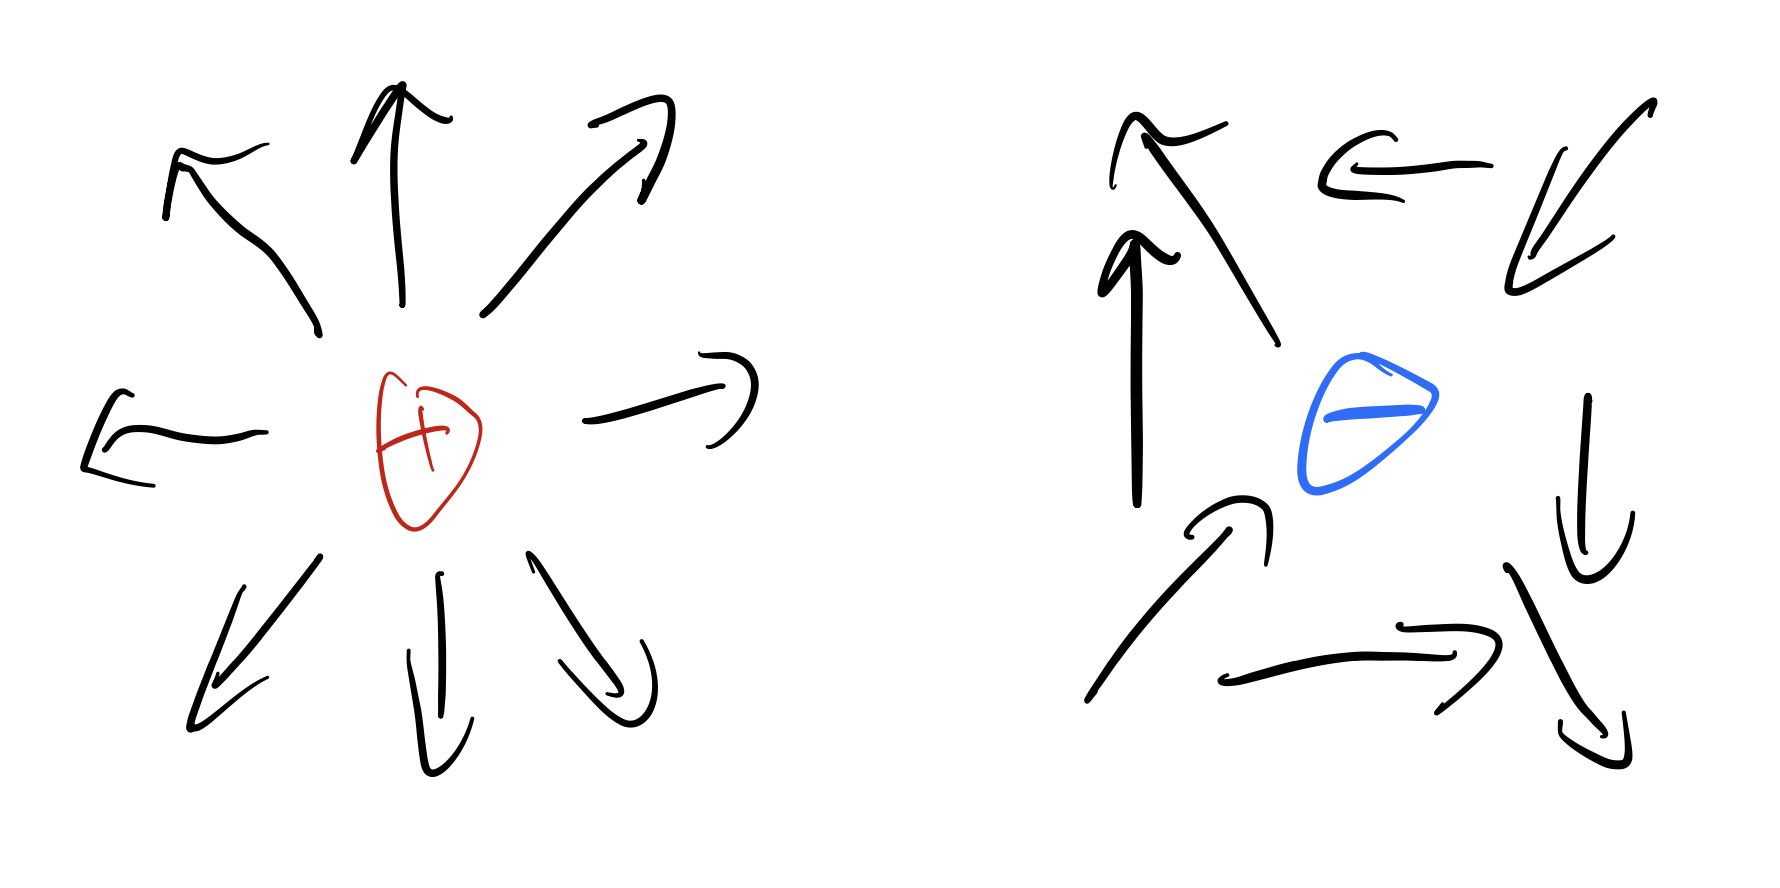
\includegraphics[scale=0.3]{Lectures/Figures/vortexcharges.png}
    \caption{Cartoon picture of spin vortex charges}
    \label{fig:vortexcharges}
\end{figure}

We can ask; does it make sense that as we go down to low $T$ we have the spontaneous formation of these vortices? Normally, one would think that it takes finite energy to place them in the lattice (so they should go away at low $T$) but there are so many places to put them and as such there is an entropic gain as well... What happens is (even at low $T$) fluctuations create charges out of a vacuum, but they will be close together and be bound. This is one phase. There is also a second possible phase where the charges unbind; we go from vortex charge molecules to a plasma; they begin to overlap, and they start screening, and the system breaks itself up. We can describe this with classical EM. This transition/plasma phase has no long range order, but the confined phase has a quasi-long range order, where the effective stiffness stays finite. The transition between these two is the Berezinskii-Kosterlitz-Thouless transition.